\section{Crystal structure of sodium chloride (NaCl)}
\label{sec:NaCl}

In the following section, we are going to examine the crytsal structure of NaCl. Using the setup described in~\ref{chap:methods} we recieved the measured intensities as function of the angle $2\theta$. The corresponding graph is shown in fig. 

\begin{figure}[ht]
    \centering
    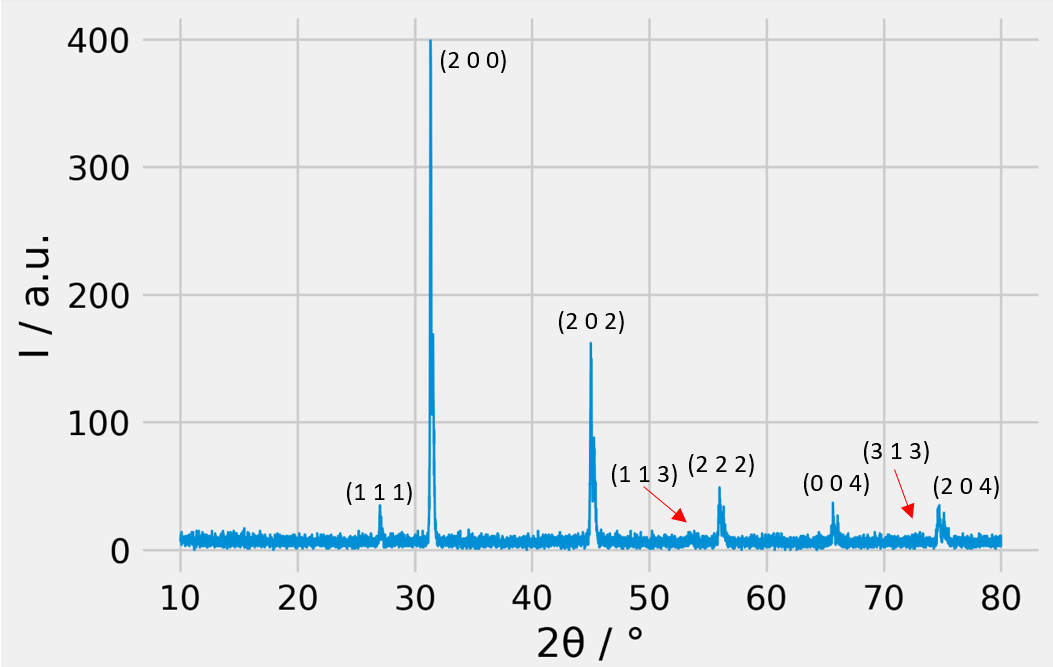
\includegraphics[angle = 90, width = 0.95\linewidth]{Bilder/Auswertung/NaCl/Ivs2thwIndices.png}
    \label{fig:Elements}
    \caption{Wavelength of the K-edge for different elements with increasing ordinal number. From (ref)}
\end{figure}
